\documentclass[twoside=false, DIV=14]{scrartcl}

\usepackage{arev} % order matters, putting this above allows FiraSans to override it for body text
\usepackage[sfdefault]{FiraSans}
\usepackage{inconsolata}
%\usepackage[fira]{fontsetup}
\usepackage{scrlayer-scrpage}
\renewcommand{\titlepagestyle}{scrheadings}
\usepackage{graphicx}
\usepackage{blindtext}
\usepackage{wrapfig}
\usepackage{tabularx}
\usepackage{hyperref}
\usepackage{listings}
\usepackage{tikz}
\usepackage{amsmath}
\usepackage[many]{tcolorbox}

\usepackage{xcolor,sectsty}
\definecolor{blackish}{RGB}{56,58,54}
\definecolor{redish}{RGB}{109,41,49}
\definecolor{red}{RGB}{152,41,50}
\definecolor{orangeish}{RGB}{188,71,0}
\definecolor{blueish}{RGB}{25,33,139}
\subsubsectionfont{\color{blackish}}
\subsectionfont{\color{blackish}}
\sectionfont{\color{blackish}}

\lohead{\color{red} COMP3000 Programming Languages}
\rohead{
\includegraphics[width=0.5cm]{../logo.jpg}}

\setkomafont{author}{\sffamily \small}
\setkomafont{date}{\sffamily \small}

\DeclareOldFontCommand{\bf}{\normalfont\bfseries}{\mathbf}
\DeclareOldFontCommand{\tt}{\normalfont\ttfamily}{\texttt}

\lstset{basicstyle=\ttfamily}


\date{}
\newtcolorbox{aside}[1][]{
  title=Aside,
  width=0.3\textwidth,
  fonttitle=\bfseries,
  breakable,
  fonttitle=\bfseries\color{black},
  colframe=blueish!80,
  colback=blueish!2
  #1}

\newtcolorbox{note}[1][]{
  title=Note,
  width=\textwidth,
  fonttitle=\bfseries,
  breakable,
  fonttitle=\bfseries\color{black},
  colframe=orangeish!80,
  colback=orangeish!2
  #1}

\newtcolorbox{hint}[1][]{
    title=Hint,
    width=\textwidth,
    fonttitle=\bfseries,
    breakable,
    fonttitle=\bfseries\color{white},
    colframe=blueish!80,
    colback=blueish!2
    #1}

\newtcolorbox{todo}[1][]{
  title=!! TODO !!,
  width=\textwidth,
  fonttitle=\bfseries,
  breakable,
  fonttitle=\bfseries\color{white},
  colframe=red!80,
  colback=red!2
  #1}
  
\providecommand{\tightlist}{%
  \setlength{\itemsep}{0pt}\setlength{\parskip}{0pt}}

\title{\color{redish} \vspace{-1em}COMP3000 Week 2: Introduction to Programming Languages}

\begin{document}
{\color{blackish}\maketitle}\vspace{-7em}

\begin{abstract}
  This week we begin our journey with programming languages, reading the introduction of our text book.
\end{abstract}

\section*{Topics}
\begin{description}
\item[The concept of little languages]  What is a little language?  Why do we care?  What are some examples?
\item[The Compiler/Interpreter Pipeline]  What is the compiler/interpreter pipeline?  What are the parts of a compiler?  What are the parts of an interpreter?  How do they differ?
\item[Compilers vs Interpreters]  What is the difference between a compiler and an interpreter?  What are some examples of each?
\end{description}
\section*{Preparation}
\begin{itemize}
\item Read the text chapters 1 and 2
\item Watch the three lectures: 
\begin{enumerate}
\item The concept of little languages
\item The compiler interpreter pipeline
\item Compilers vs Interpreters.
\end{enumerate}
\item Complete the RAT individually \emph{and} bring your answers to class.
\end{itemize}

\section*{Definitions to help while preparing}
\begin{description}
\item[pidgins]: A language with simplified grammar from another language and lots of loan-words from native languages.  My favourite is Tok Pisin.
\item[sound]: If you follow these rules, you won't do anything wrong
\item[complete]: If you follow these rules, you won't miss anything.
\item[stream]: Like an array or Vector but it arrives over time, not all at once.  \emph{Files} are commonly treated as streams because it takes time to get them from the hard drive and they might be much bigger than your memory.
\end{description}

\newpage
\part*{RAT 2 \hspace{6em} {\small INDICATE YOUR RESPONSE TO EACH QUESTION}}
\RAT
\begin{enumerate}
\item \textbf{Which of these characteristics would make a language implementation \emph{certainly} a compiler:}
\begin{enumerate}
  \item code generation \tick
  \item scanning
  \item parsing
  \item interpretation
  \item static analysis
\end{enumerate}

\item \textbf{Which of the following is a synonym for \emph{lexing}:}
\begin{enumerate}
  \item parsing
  \item scanning \tick
  \item luthering
  \item code generation
  \item interpretation
  \item static analysis
\end{enumerate}

\item \textbf{At which point does the language's semantics start to come into play?}
\begin{enumerate}
  \item parsing
  \item scanning
  \item code generation
  \item interpretation
  \item static analysis \tick
\end{enumerate}

\item \textbf{Which of the following are optimisations a compiler/interpreter might do?}
\begin{enumerate}
  \item change \lstinline|"five"| to \lstinline|5|
  \item change \lstinline|5 + 5| to \lstinline|10| \tick
  \item change \lstinline|5 + 5| to \lstinline|10 + 0|
  \item strip \lstinline|if true| from a block of code \tick
  \item remove a loop that executes zero times \tick
  \item convert from an $O(n^2)$ algorithm to an $O(n)$ algorithm.
\end{enumerate}

\item \textbf{Two of the following phases can't easily co-exist in a single compiler/interpreter.  Which two?}
\begin{enumerate}
  \item code generation \tick
  \item scanning
  \item parsing
  \item interpretation \tick
  \item static analysis
\end{enumerate}
\end{enumerate}

\newpage
\part*{Application Exercise}
Regular Expressions are a very popular "little language" for pattern matching in text.  In this exercise your group will explore regular expressions and at the end of class will:
\begin{itemize}
  \item Show off your most "fun" regular expression.
  \item Decide if regular expressions qualify as a "complete" language and explain your reasoning.
\end{itemize}
It is up to you and your group to work towards these goals however you like but we suggest the following subtasks which naturally lead to the goals:
\begin{enumerate}
  \item Go to \verb+https://regexr.com+.
  \item Come up with an example string.  I used {\tiny \begin{quote} GEORGE: The sea was angry that day my friends, like an old man trying to send back soup in a deli. I got about fifty-feet out and then suddenly the great beast appeared before me. I tell ya he was ten stories high if he was a foot. As if sensing my presence he gave out a big bellow. I said, "Easy big fella!" And then as I watched him struggling I realized something was obstructing his breathing. From where I was standing I could see directly into the eye of the great fish! JERRY: Mammal. GEORGE: Whatever. KRAMER: Well, what did you do next? GEORGE: Then from out of nowhere a huge title wave lifted, tossed like a cork and I found myself on top of him face to face with the blow-hole. I could barely see from all of the waves crashing down on top of me but I knew something was there so I reached my hand and pulled out the obstruction!\end{quote}}
  \item Test looking for some particular exact string.  I looked for "my presence".
  \item Test looking for one of two strings. I looked for "my presence" or "my friends".
  \item Test looking for a repeated string.  I looked for repeated p's or repeated g's or repeated l's.
  \item Try to "capture" a match for use elsewhere.  I looked for the first word used by each character at the start of their dialogue.
  \item Try to identify each of: variables, loops, conditions, and functions within regular expression syntax.
\end{enumerate}

\section*{On Completeness}
A language is "complete" if it can express all possible computations.  All complete languages thus have equivalent expressive power, even though we might find some much easier to use than others.  Knowing \emph{for sure} if a language is complete can take some maths nouse, but we can get a good approximation by looking for certain lanuage feeatures:
\begin{itemize}
  \item \textbf{Variables, Conditions, Loops}: A language with variables, conditions, and loops is probably complete.  This is the "Turing" view of completeness and corresponds to a turing machine.
  \item \textbf{Variables, Functions}: A language with variables and functions is probably complete.  This is the "Church" view of completeness and corresponds to a computational calculus\footnote{This dual nature of computing is one of the most fascinating aspects of programming language theory.  Some fundamental truths of the universe are hidden within it}.
\end{itemize}

\newpage
\part*{Application Exercise Notes and Solutions}
I wanted to find all the first words used by each Seinfeld character in the scene.  I loaded up all the script from the episode "The Non-Fat Yoghurt".

To get all the first words used by Kramer I used the regex \verb|Kramer\s*([A-z]*)| which got me these words: So, Yeah, Yeah, Well, Yeah, Yes, Hey, Yow, Well, I, Yeah, I, No, Well, You, You, Oh, What, Hey, Giddy, Well, It, Hey, Hello, Ooh, Well, Why, I, Where, Yeah, I, Well, Well, Hey, Well, No
You, He, Yeah, He, Yeow, Okay
Mine, Yeah.

I did the same for George and got these words: Fantastic, Good, Very, See, Oh, Okay, What, No, Oh, This, Hey, Yeah, Uh, Oh, Yeah, Uh, Yeah, He, All, No, What, Hey, yesterday, Oh, Nothing, Yeah, Well, with, You, All, Oh, Oh, Yeah, So, And, I, Oh, Oh, Why, So, Already, All, Yeah, The, Please, Yes, Uh, Hmm, Well, How, Faking, Now, Fine, Name, I, Phew

Which I thought was quite interesting.  You can see that good script writing means even the very first words of a character are carefully chosen to give you a sense of their character.  

\subsection*{On Completeness}
I found variables in the form of capture groups which you can use again later.  I found loops in the form of \verb|*| and \verb|+| but I am not convinced on conditions.  The \verb|?| operator certainly looks like a condition but it can't change the flow of computation, so I am unsure.  I didn't find anything that looked like a function.

On balance, I think regular expressions are not complete.  If I ask the internet for an answer I find out some variants of regular expressions are complete and others are not - which matches with my vibe from my investigation.
\newpage
\part*{Self Study Exercises}
\section*{Text Exercises}
Complete challenge 1 and 2 from  Chapter 1 of the text.

\section*{Pick a Little Language}
Find a "little language" you have used somewhere.

\subsection*{Solution}
  The command language in minecraft is \emph{almost} a little language but it does not include any control flow so perhaps that is being generous?  Though redstone can get you control flow.  Little languages are often very restricted and rely on machinery from elsewhere to do the hard work, so I think it counts in the end.  More likely you will have used BASH, which is the little language you use whenever you do something in the command line.  It has heaps of features you never thought to use.

  \section*{Counting Branches}
Imagine the following diagram of programming language implementation options is \emph{sound} and \emph{complete}.  We want to create a compiler/interpreter to convert our "source" language into one of our target languages (x86 or ARM).
  
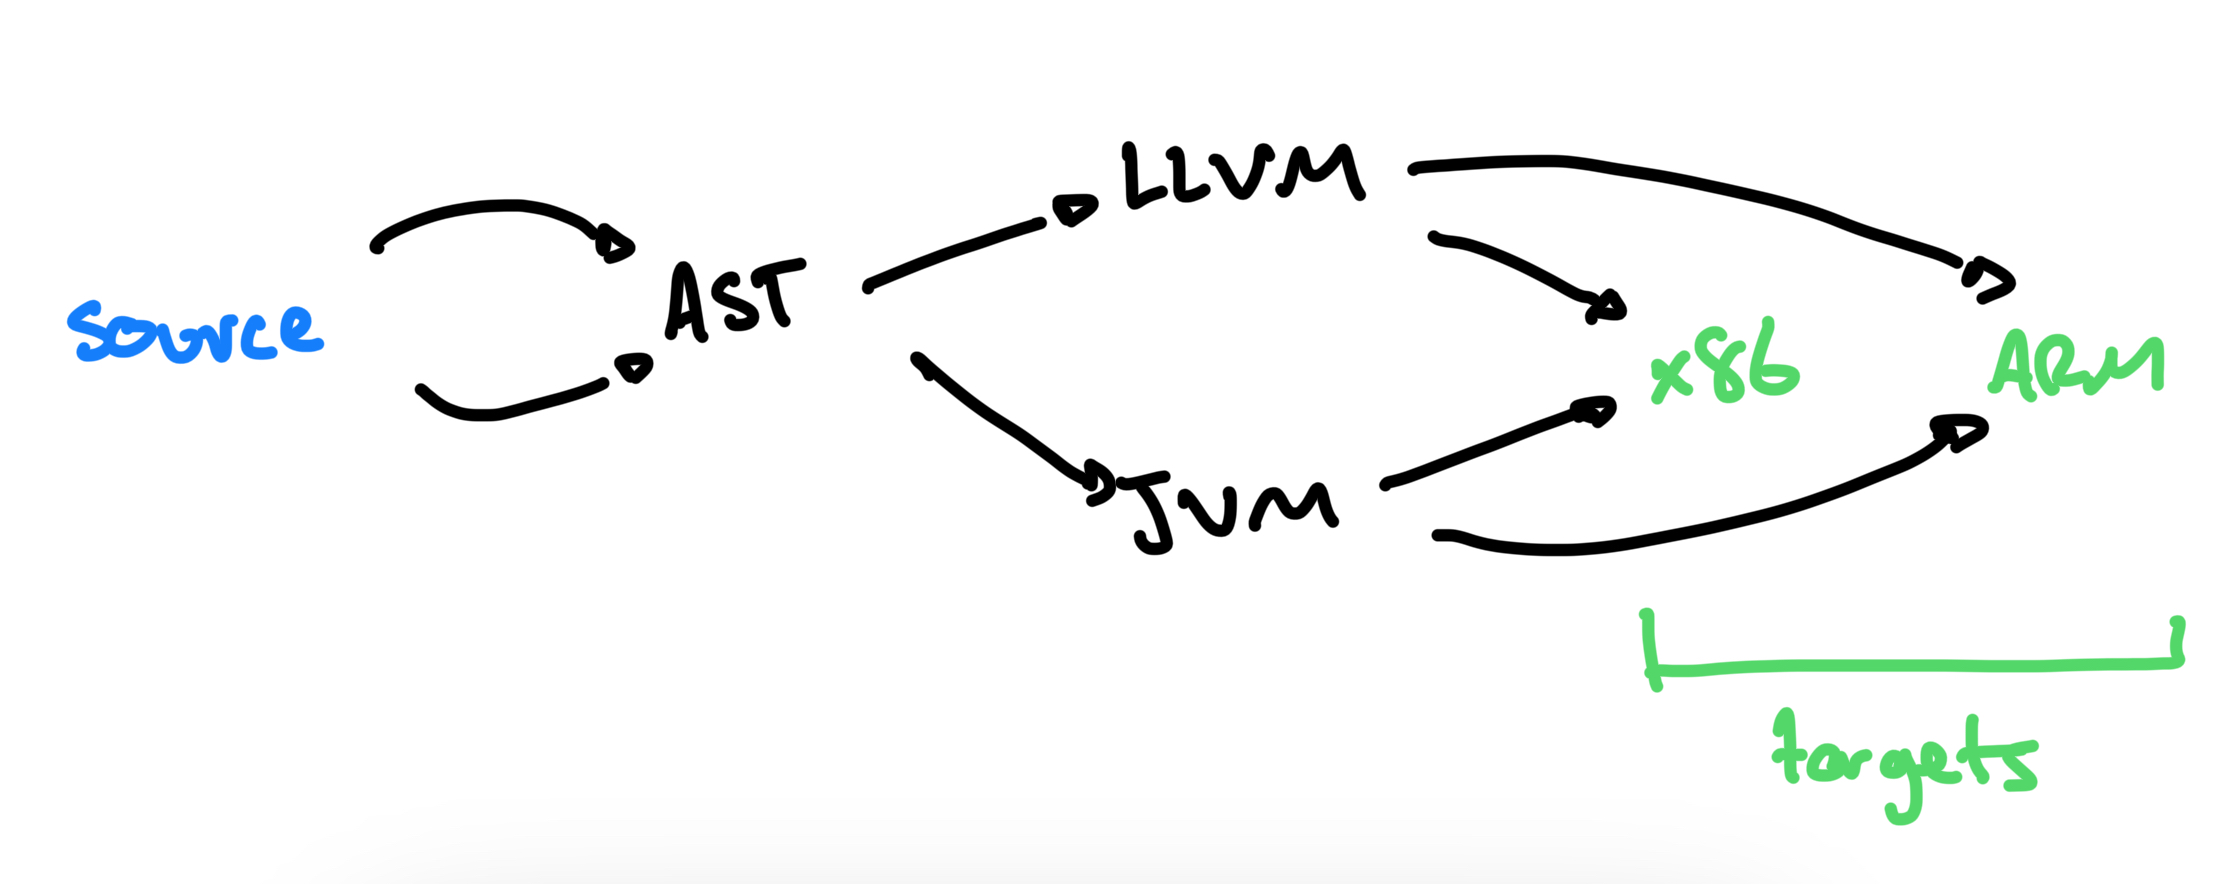
\includegraphics[width=0.5\textwidth]{2_paths.jpeg}

How many different possible implementations are there? (Hint, this is a COMP2010 question)

\section*{Compiler Parts}
\begin{minipage}[t]{0.4\textwidth}
Match these compiler parts 
\begin{itemize}
  \item code generation 
  \item parser 
  \item scanner
  \item optimization
  \item static analysis
\end{itemize}
\end{minipage}
\hspace{2em}
\begin{minipage}[t]{0.4\textwidth}
with a description of what they do:
\begin{itemize}
  \item takes in the linear stream of characters and chunks them together into a series
  \item takes the flat sequence of tokens and builds a tree structure that mirrors the nested nature of the grammar
  \item get a high-level view of what the code is doing
  \item remove redundancy and do early computation
  \item output machine code
\end{itemize}
\end{minipage}

\section*{Solution}
\begin{description}
  \item[scanner] takes in the linear stream of characters and chunks them together into a series
  \item[parser] takes the flat sequence of tokens and builds a tree structure that mirrors the nested nature of the grammar
  \item[static analysis] get a high-level view of what the code is doing
  \item[optimisation] remove redundancy and do early computation
  \item[code generation] output machine code
\end{description}
\section*{Language Classification}
  Discuss which of the following are compilers and which are interpreters:
  \begin{itemize}
    \renewcommand{\labelitemi}{$\square$}
    \item Java
    \item JavaScript
    \item Processing
    \item C
  \end{itemize}
  
\subsection*{Solution}
Key to this question is that these are languages, and we can't answer for languages. We can only answer for particular language implementations! However, most languages come with standard implementations \emph{or} the implementations all use the same general approach. For Java and Processing and C, all implementations are compilers (though processing is a "transpiler"). For JavaScript, there are \emph{both} compiled and interpreted implementations.

\section*{Compiler or Interpreter?}
In your own words, give \emph{a single sentence} that describes \emph{the most important} distinction between compilers and interpreters.

\subsection*{Solution}
Compilers will output code, probably in a lower-level language, while interpreters will execute the code directly.

\section*{Regex}
  Write a regular expressions that will work over the following text to extract:
  \begin{itemize}
    \item every instance of "the the" and "teh" (common errors)
    \item The last word of every sentence
    \item All characters in the scene
    \item All the scene directives
  \end{itemize}

  \begin{quote}
  (Opening scene:  A table golf set.  As the camera pulls back, CAT's head
  rises into view over the edge of the the table.  He is wearing a rather
  ridiculous multi-coloured tammy, a red golfing jumper with a large 'Red
  Dwarf' badge and garish plus fours.  He is carefully lining up a shot.)
  
  CAT: (Rising) Okay, okay, okay.  Uphill, slight barrow to the left.
   
  (He pulls back the club on his miniature golfer, causing it to putt the
  ball into the hole.)
   
  CAT: (Ecstatic) Yes, yes, yes, YES!  Yow!
   
  (He switches on a tape recorder sitting beside the scaled-down green.
  Cheering and applause emerge from the speakers.  CAT bows and blows
  kisses happily.  The camera pans to teh right, and we see LISTER, who is
  sitting with arms folded, looking rather unhappy.)
   
  CAT: (In LISTER's face) Yay!  Four up, with six to play!  This guy is
  hot, hot, HOT!  Okay, hole 13.
  LISTER: What am I doing?  What am I doing here?
  CAT: You're not following through is what you're doing!  Keep your head
  down and follow through!
  \end{quote}
\subsection*{Solution}
\begin{itemize}
  \item \lstinline`/(the the|teh)/`
  \item \lstinline`/\S[A-z]*\./`
  \item \lstinline`/^[A-Z]*:/`
  \item \lstinline`/\([\S\s]*\)/gmU`
\end{itemize}



\section*{Exits}
  There are multiple end-points for the paths over the crafting interpreters mountain, what are they?
\subsection*{Solution}
    \begin{itemize}
      \item High level language
      \item Bytecode
      \item Machine Code
    \end{itemize}


\section*{Combining Optimisations}
  There is an optimisation called \emph{constant propagation} which notices if a variable never changes and replaces all instances of that variable with the value it will always have. The textbook talked about \emph{constant folding}. Can you think of a program (in whatever language you like) where \emph{constant propagation} might open up new opportunities to do \emph{constant folding}?
\subsection*{Solution}
  Here is mine (in Ruby):
  \begin{verbatim}
  x = 5  \# x is a constant and never changes
  puts 5 * x
  \end{verbatim}
  The \texttt{5 * x} is not ready for constant folding \emph{until} we realize the \texttt{x} will always be \texttt{5}, then the program can be transformed to:
  \begin{verbatim}
  puts 5 * 5
  \end{verbatim}
  Which can be optimized with constant folding to:
  \begin{verbatim}
  puts 25
  \end{verbatim}

\section*{Tree Walker}
Which of the following phases would be left out of a "tree walk interpreter"?
\begin{itemize}
    \item scanner
    \item code generation
    \item runtime
    \item parsing
\end{itemize}
\subsection*{Solution}
Code generation and runtime would be left out of a tree walker.  The tree walker is a kind of interpreter that does not generate code, it just walks the tree and executes the code as it goes.  The scanner and parser are still needed to get the tree in the first place.

section*{Transpiler}
Which of the following phases would be left out of a "transpiler"?
\begin{itemize}
    \item scanner
    \item code generation
    \item runtime
    \item parsing
\end{itemize}
\subsection*{Solution}
Runtime would be left out of a transpiler.  A transpiler still generates code, it just generates it in another high-level language.

\section*{Hypothetical}
  If I told you I had a program which did a "quick and dirty" conversion from BASH script to Ruby, would you think it was a compiler or an interpreter?  Justify your choice.
  \subsection*{Solution}
  This would have to be a compiler! It \emph{sounds like} an interpreter because it is "quick and dirty, " but it doesn't actually run any code! It takes code in a source language and converts it to another language. It just so happens the "other" language is commonly used as a source language. Even the assembly code you are used to generating in a compiler is actually run through an interpreter in the end (really, it is true), so having Ruby as a target language is not so strange after all.

\section*{Real Interpreter}
What is a programming language implementation you know of that \emph{certainly} is an interpreter rather than a compiler?

  \subsection*{Solution}
  The text identifies early versions of Ruby. I will nominate \texttt{sed}, which performs stream editing on Unix. \texttt{sed} has a configuration language that qualifies as a domain-specific language for making changes to a text file.

\section*{Why not Langauge?}
In your own words, explain why is is not meaningful to ask if a language is compiled or interpreted.

\subsection*{Solution}
A language is a set of rules for writing programs.  A program is a set of instructions for a computer to follow.  A compiler or interpreter is a program that takes a program in one language and converts it to another language.  So the question is not meaningful because it is asking about the wrong thing.  It should be asking about the implementation of the language, not the language itself.  

However, all the implementations of a particular language are usually similar, so it is common to talk about a language as if it is a single thing.  This is not strictly correct, but it is a useful simplification.  It is also common to talk about the "compiler" or "interpreter" of a language as if it is a single thing, even though there are many different implementations of each.

Languages where all implementations are interpreters are Ruby, BASH, and R.  Languages where all implementations are compilers are Java, C, and Processing.  Languages where there are both interpreters and compilers are JavaScript and Python\footnote{As long as we include CPython as real python, which is disputed}.
\end{document}